% ========================================
%	Header einbinden
% ========================================

\documentclass[bibtotoc,titlepage]{scrartcl}

% Deutsche Spracheinstellungen
\usepackage[ngerman,german]{babel, varioref}
\usepackage[T1]{fontenc}
\usepackage[utf8]{inputenc}

%\usepackage{marvosym}

\usepackage{amsfonts}
\usepackage{amssymb}
\usepackage{amsmath}
\usepackage{amscd}
\usepackage{amstext}

\usepackage{longtable}

%\usepackage{bibgerm}

\usepackage{footnpag}

\usepackage{ifthen}                 %%% package for conditionals in TeX
\usepackage[amssymb]{SIunits}
%Für textumflossene Bilder und Tablellen
%\usepackage{floatflt} - veraltet

%Für Testzwecke aktivieren, zeigt labels und refs im Text an.
%\usepackage{showkeys}

% Abstand zwischen zwei Absätzen nach DIN (1,5 Zeilen)
% \setlength{\parskip}{1.5ex plus0.5ex minus0.5ex}

% Einrückung am Anfang eines neuen Absatzes nach DIN (keine)
%\setlength{\parindent}{0pt}

% Ränder definieren
% \setlength{\oddsidemargin}{0.3cm}
% \setlength{\textwidth}{15.6cm}

% bessere Bildunterschriften
%\usepackage[center]{caption2}


% Problemlösungen beim Umgang mit Gleitumgebungen
\usepackage{float}

% Nummeriert bis zur Strukturstufe 3 (also <section>, <subsection> und <subsubsection>)
%\setcounter{secnumdepth}{3}

% Führt das Inhaltsverzeichnis bis zur Strukturstufe 3
%\setcounter{tocdepth}{3}
\usepackage[version=3]{mhchem}
	\mhchemoptions{minus-sidebearing-left=0.06em, minus-sidebearing-right=0.11em}
\usepackage{exscale}

\newenvironment{dsm} {\begin{displaymath}} {\end{displaymath}}
\newenvironment{vars} {\begin{center}\scriptsize} {\normalsize \end{center}}


\newcommand {\en} {\varepsilon_0}               % Epsilon-Null aus der Elektrodynamik
\newcommand {\lap} {\; \mathbf{\Delta}}         % Laplace-Operator
\newcommand {\R} { \mathbb{R} }                 % Menge der reellen Zahlen
\newcommand {\e} { \ \mathbf{e} }               % Eulersche Zahl
\renewcommand {\i} { \mathbf{i} }               % komplexe Zahl i
\newcommand {\N} { \mathbb{N} }                 % Menge der nat. Zahlen
\newcommand {\C} { \mathbb{C} }                 % Menge der kompl. Zahlen
\newcommand {\Z} { \mathbb{Z} }                 % Menge der kompl. Zahlen
\newcommand {\limi}[1]{\lim_{#1 \rightarrow \infty}} % Limes unendlich
\newcommand {\sumi}[1]{\sum_{#1=0}^\infty}
\newcommand {\rot} {\; \mathrm{rot} \,}         % Rotation
\newcommand {\grad} {\; \mathrm{grad} \,}       % Gradient
\newcommand {\dive} {\; \mathrm{div} \,}        % Divergenz
\newcommand {\dx} {\; \mathrm{d} }              % Differential d
\newcommand {\cotanh} {\; \mathrm{cotanh} \,}   %Cotangenshyperbolicus
\newcommand {\asinh} {\; \mathrm{areasinh} \,}  %Area-Sinus-Hyp.
\newcommand {\acosh} {\; \mathrm{areacosh} \,}  %Area-Cosinus-H.
\newcommand {\atanh} {\; \mathrm{areatanh} \,}  %Area Tangens-H.
\newcommand {\acoth} {\; \mathrm{areacoth} \,}  % Area-cotangens
\newcommand {\Sp} {\; \mathrm{Sp} \,}
\newcommand {\mbe} {\stackrel{\text{!}}{=}}     %Must Be Equal
\newcommand{\qed} { \hfill $\square$\\}
\renewcommand{\i} {\imath}
\def\captionsngerman{\def\figurename{\textbf{Abb.}}}

%%%%%%%%%%%%%%%%%%%%%%%%%%%%%%%%%%%%%%%%%%%%%%%%%%%%%%%%%%%%%%%%%%%%%%%%%%%%
% SWITCH FOR PDFLATEX or LATEX
%%%%%%%%%%%%%%%%%%%%%%%%%%%%%%%%%%%%%%%%%%%%%%%%%%%%%%%%%%%%%%%%%%%%%%%%%%%%
%%%
\ifx\pdfoutput\undefined %%%%%%%%%%%%%%%%%%%%%%%%%%%%%%%%%%%%%%%%% LATEX %%%
%%%
\usepackage[dvips]{graphicx}       %%% graphics for dvips
\DeclareGraphicsExtensions{.eps,.ps}   %%% standard extension for included graphics
\usepackage[ps2pdf]{thumbpdf}      %%% thumbnails for ps2pdf
\usepackage[ps2pdf,                %%% hyper-references for ps2pdf
bookmarks=true,%                   %%% generate bookmarks ...
bookmarksnumbered=true,%           %%% ... with numbers
hypertexnames=false,%              %%% needed for correct links to figures !!!
breaklinks=true,%                  %%% breaks lines, but links are very small
linkbordercolor={0 0 1},%          %%% blue frames around links
pdfborder={0 0 112.0}]{hyperref}%  %%% border-width of frames
%                                      will be multiplied with 0.009 by ps2pdf
%
\hypersetup{ pdfauthor   = {Hannes Franke; Julius Tilly},
pdftitle    = {V301 Innenwiderstand und Leistungsanpassung}, pdfsubject  = {Protokoll FP}, pdfkeywords = {V301, Innenwiderstand, Leistungsanpassung},
pdfcreator  = {LaTeX with hyperref package}, pdfproducer = {dvips
+ ps2pdf} }
%%%
\else %%%%%%%%%%%%%%%%%%%%%%%%%%%%%%%%%%%%%%%%%%%%%%%%%%%%%%%%%% PDFLATEX %%%
%%%
\usepackage[pdftex]{graphicx}      %%% graphics for pdfLaTeX
\DeclareGraphicsExtensions{.pdf}   %%% standard extension for included graphics
\usepackage[pdftex]{thumbpdf}      %%% thumbnails for pdflatex
\usepackage[pdftex,                %%% hyper-references for pdflatex
bookmarks=true,%                   %%% generate bookmarks ...
bookmarksnumbered=true,%           %%% ... with numbers
hypertexnames=false,%              %%% needed for correct links to figures !!!
breaklinks=true,%                  %%% break links if exceeding a single line
linkbordercolor={0 0 1},
linktocpage]{hyperref} %%% blue frames around links
%                                  %%% pdfborder={0 0 1} is the default
\hypersetup{
pdftitle    = {V301 Innenwiderstand und Leistungsanpassung}, 
pdfsubject  = {Protokoll AP}, 
pdfkeywords = {V301, Innenwiderstand, Leistungsanpassung},
pdfsubject  = {Protokoll AP},
pdfkeywords = {V301, Innenwiderstand, Leistungsanpassung}}
%                                  %%% pdfcreator, pdfproducer,
%                                      and CreationDate are automatically set
%                                      by pdflatex !!!
\pdfadjustspacing=1                %%% force LaTeX-like character spacing
\usepackage{epstopdf}
%
\fi %%%%%%%%%%%%%%%%%%%%%%%%%%%%%%%%%%%%%%%%%%%%%%%%%%% END OF CONDITION %%%
%%%%%%%%%%%%%%%%%%%%%%%%%%%%%%%%%%%%%%%%%%%%%%%%%%%%%%%%%%%%%%%%%%%%%%%%%%%%
% seitliche Tabellen und Abbildungen
%\usepackage{rotating}
\usepackage{ae}
\usepackage{
  array,
  booktabs,
  dcolumn
}
\makeatletter 
  \renewenvironment{figure}[1][] {% 
    \ifthenelse{\equal{#1}{}}{% 
      \@float{figure} 
    }{% 
      \@float{figure}[#1]% 
    }% 
    \centering 
  }{% 
    \end@float 
  } 
  \makeatother 


  \makeatletter 
  \renewenvironment{table}[1][] {% 
    \ifthenelse{\equal{#1}{}}{% 
      \@float{table} 
    }{% 
      \@float{table}[#1]% 
    }% 
    \centering 
  }{% 
    \end@float 
  } 
  \makeatother 
%\usepackage{listings}
%\lstloadlanguages{[Visual]Basic}
%\allowdisplaybreaks[1]
%\usepackage{hycap}
%\usepackage{fancyunits}

\usepackage{float}
\usepackage{caption}

\newfloat{formel}{htbp}{for}
\floatname{formel}{Formel}

% ========================================
%	Angaben für das Titelblatt
% ========================================

\title{Aktivierung durch langsame Neutronen\\				% Titel des Versuchs 
\large TU Dortmund, Fakultät Physik\\ 
\normalsize Anfänger-Praktikum}

\author{Jan Adam\\			% Name Praktikumspartner A
{\small \href{jan.adam@tu-dortmund.de}{jan.adam@tu-dortmund.de}}	% Erzeugt interaktiven einen Link
\and						% um einen weiteren Author hinzuzfügen
Dimitrios Skodras\\			% Name Praktikumspartner B
{\small \href{dimitrios.skodras@tu-dortmund.de}{dimitrios.skodras@tu-dortmund.de}}		% Erzeugt einen interaktiven Link
}
\date{20.11.12}					% Das Datum der Versuchsdurchführung

% ========================================
%	Das Dokument beginnt
% ========================================

\begin{document}

% ========================================
%	Titelblatt erzeugen
% ========================================

\maketitle					% Jetzt wird die Titelseite erzeugt
\thispagestyle{empty} 				% Weder Kopfzeile noch Fußzeile

% ========================================
%	Der Vorspann
% ========================================

%\newpage					% Wenn Verzeichnisse auf einer neuen Seite beginnen sollen
%\pagestyle{empty}				% Weder Kopf- noch Fußzeile für Verzeichnisse

\tableofcontents

%\newpage					% eine neue Seite
%\thispagestyle{empty}				% Weder Kopf- noch Fußzeile für Verzeichnisse
%\listoffigures					% Abbildungsverzeichnis

%\newpage					% eine neue Seite
%\thispagestyle{empty}				% Weder Kopf- noch Fußzeile für Verzeichnisse
%\listoftables					% Tabellenverzeichnis
\newpage					% eine neue Seite


% ========================================
%	Kapitel
% ========================================

	\section{Einleitung}				% Bei Bedarf
Abgesehen vom Wasserstoffatom, bestehen Atomkerne aus Protonen und Neutronen. Damit der Kern jedoch trotz der Coulombkräfte stabil bleibt, muss ein gewisses Verhältnis zwischen den Anzahlen der jeweiligen Teilchen gewahrt werden. Ändert es sich über einen bestimmten Wert hinaus, so wird der Kern instabil und zerfällt nach einer gewissen Zeit in einem oder mehreren mehreren Schritten, bis er wieder einen stabilen Zustand erreicht.
	\section{Theorie}
	\subsection{Aktivierung}
Dieses Verhalten kann für die Untersuchung des Zerfallsgesetztes genutzt werden.
Indem stabile Atomkerne mit langsamen Neutronen beschossen werden, können sich diese in andere, instabile Isotope umwandeln, deren Radioaktivität im Folgenden mit einem Geiger-Müller-Zählrohr gemessen werden kann. Dieser Vorgang wird als Aktivierung bezeichnet.\\
Interessant ist die Aktivierung insbesondere deshalb, weil sich so neues radioaktives Material mit kurzen Halbwertszeiten herstellen lässt, welches wegen seinem schnelleren Zerfall nicht gelagert werden kann.
Die Wahl von Neutronen ist günstig, denn aufgrund ihrer fehlenden Ladung müssen sie nicht nicht die Coulombkräfte des Kerns überwinden um eine Kernreaktion herbeizuführen. Für geladene Teilchen sind hier Energien im Bereich von 10MeV nötig, die nur in Teilchenbeschleunigern erreicht werden können. Neutronen mit der benötigten kinetischen Energie können dagegen problemlos im Labor durch Zerfall anderer radioaktiver Stoffe erzeugt werden.\\
Geht das Neutron eine Reaktion mit dem Atomkern A ein, so entsteht ein neuer Kern A* auch Zwischenkern genannt, dessen Energie um den Betrag der kinetischen und der Bindungsenergie den Neutrons höher ist als die Energie des Kerns A. Dies wird auch als Aufheizen des Zwischenkerns bezeichnet. Da die Nukleonen starken Wechselwirkungen unterliegen, verteilt sich die aufgenommene Energie jedoch sofort und keines der angeregten Nukleonen hat genug Energie um den Kern direkt wieder zu verlassen. Da es energetisch günstiger ist, wird deshalb nach etwa $10^{-16}$s ein $\gamma$-Quant abgestrahlt und der Kern geht wieder in seinen Grundzustand über.\\
Es läuft somit folgende Reaktion ab:
\begin{formel}
\begin{equation}
	{\ce{^m_z A + ^1_0 n -> ^{m+1}_z A^* -> ^{m+1}_z A +\gamma}} 
\end{equation}
\caption*{m = Massenzahl}
\end{formel}
\\
Der neu entstandene Kern ist normalerweise nicht stabil, da er ein Neutron zuviel besitzt, ist jedoch aufgrund des Energieverlusts durch das $\gamma$-Quant relativ langlebig. Schließlich wandelt er sich aber durch Aussendung eines Elektrons ($\beta^-$-Strahlung) in einen stabilen Kern um
\begin{align}
	\ce{^{m+1}_zA -> ^{m+1}_{z+1}C +\beta^- +\overline{\nu_e} + E_{kin}}.
\end{align}
Der Ausgangskern ist leichter als die Summe aller Zerfallprodukte, da ein Teil der Masse in Form von Bindungsenergie zwischen den Nukleonen vorlag. Die Bindungsenergie, die beim Umwandeln frei wird, wird gemäß der Einsteinschen Beziehung
\begin{align}
	\Delta E = \Delta mc^2
\end{align}
als kinetische Energie an das Elektron bzw. das Antineutrino abgegeben.\\
Wichtig für den durchgeführten Versuch sind insbesondere die Zerfallsreihen von $\ce{^{116}Indium}$ und $\ce{^{104}Rhodium}$
\begin{align}
\cee{^{115}_{49} In +^1_0n -> ^{116}_{49}In -> ^{116}_{50}Sn +\beta- + \overline{\nu_e}}\\
\vspace{0.5cm}
\cee{^{103}_{45}Rh +^1_0n } 
\begin{cases} \ce{->[{10\%}] ^{104i}_{45}Rh -> ^{104}_{45}Rh +\gamma -> ^{104}_{46}Pd + \beta^- + \overline{\nu_e}}\\ 
\cee{ ->[{90\%}] ^{104}_{45}Rh -> ^{104}_{46}Pd + \beta^- + \overline{\nu_e}} \end{cases}
\end{align}

	\subsection{Wirkungsquerschnitt}
Kernreaktionen finden zufällig statt und können nicht vorhergesagt werden. Aus diesem Grund wird in der Kernphysik der Wirkungsquerschnitt
\begin{align}
	\sigma= \frac{u}{nKd}
\end{align}
eingeführt. Dieser beschreibt die Querschnittsfläche, die das Atom haben müsste, damit jedes Neutron, welches diese Fläche passiert, auch vom Kern eingefangen wird. Der Wirkungsquerschnitt verhält sich zudem antiproportional zu der Geschwindigkeit der Neutronen. Je langsamer ein Neutron ist, desto höher ist die Wahrscheinlichkeit, dass es zu einer Kernreaktion kommt, da sich das Neutron so zu sagen länger im Einzugsbereich des Kerns aufhält. Charakteristisch ist hier insbesondere die De-Broglie-Wellenlänge $\lambda$. Sie errechnet sich für Neutronen zu
\begin{align}
	\lambda=\frac{\hbar}{m_n v}.
	\label{broglie}
\end{align}
Wegen des Welle-Teilchen-Dualismus kann jedes Teilchen auch als Welle mit einer Wellenlänge nach \ref{broglie} betrachtet werden. Solange $v_n$ so groß ist, dass $\lambda \ll R$ ({\small R= Kerndurchmesser}) ist, überwiegt der Teilchencharakter der Neutronen und die Trefferwahrscheinlichkeit kann geometrisch errechnet werden. Wird jedoch $\lambda \geq R$, so tritt der Wellencharakter in den Vordergrund und am Atomkern treten Interferenzeffekte auf. Nach Breit und Wigner verhält sich der Wirkungsquerschnitt in Abhängigkeit von der Energie des Neutrons wie folgt:
\begin{align}
	\sigma (E) = \sigma_0 \sqrt{\frac{{R_r}_i}{E}} \frac{\tilde c}{(E-{E_r}_i)^2 	+ \tilde c}
\end{align}
Für kleine Geschwindigkeiten folgt
\begin{align}
	\sigma \propto \frac{1}{\sqrt{E}} \propto \frac{1}{v},
\end{align}
was vorher auch schon argumentativ angenommen wurde.
	\subsection{Langsame Neutronen}
Neutronen sind als freie Teilchen instabil und kommen deshalb in der Natur nicht vor. Um sie für die Aktivierung von Atomkernen zu nutzen, müssen sie somit zunächst durch andere Radioaktive Zerfälle erzeugt werden. Im Versuch geschieht dies durch den Beschuss von $\ce{^9Be}$ mit $\alpha$-Teilchen
\begin{align}
	\ce{^9_4 Be + ^4_2\alpha \bond{->} ^{12}_6 c + ^1_0n}
\end{align}
Es entstehen Neutronen mit einem kontinuierlichen Energie-Spektrum von bis zu 13,7MeV, die abgebremst werden, indem man sie elastisch mit anderen leichten Kernen stoßen lässt. Das $\ce{^9_4 Be}$ befindet sich in einem Tank mit Wasserstoff, da diese in etwa die gleiche Masse wie Neutronen haben und daher die übertragene Energie $E = E_0 \frac{4Mm}{(M+m)^2}$ für den elastischen Stoß maximal wird.
\begin{figure}[H]
	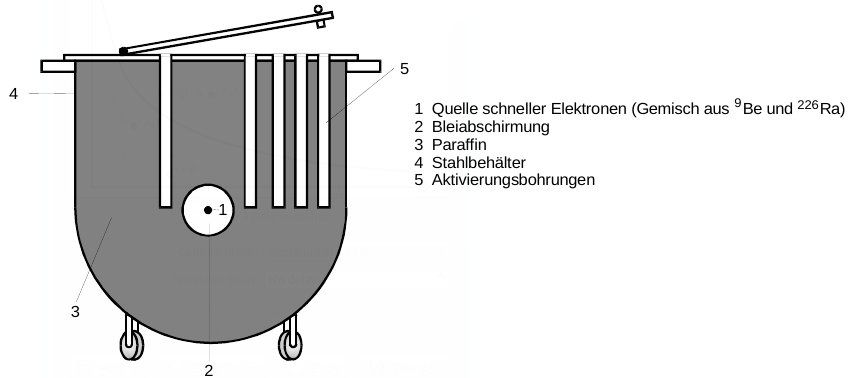
\includegraphics[scale=0.45]{pics/aktivator.jpeg}
	\caption{Querschnitt durch den Aktivator-Tank - entnommen aus der Versuchsanleitung}
\end{figure}
Die Neutronen erreichen schließlich eine mittlere Geschwindigkeit von 2,2 $\frac{km}{s}$. Neutronen mit dieser kinetischen Energie werden auch thermische Neutronen genannt.
	\subsection{Zerfallsgesetz}
\begin{align}
	N(t)=N_0e^{-\lambda t}
	\label{zerfall}
\end{align}
beschreibt die Anzahl der noch nicht zerfallenen Kerne eines radioaktiven Stoffes. Dabei ist $N_o$ die Anfangsstoffmenge und $\lambda$ die sog. Zerfallskonstante, die stoffspezifisch ist und angibt, wie schnell ein Stoff zerfällt. Da radioaktiver Zerfall zufällig stattfindet, kann man nur Aussagen über größere Stoffmengen machen und führt daher die Halbwertszeit ein, nach der von einem Stoff nur noch die Hälfte des ursprünglichen Materials vorhanden ist. Sie errechnet sich nach dem Ansatz
\begin{align}
	\frac{1}{2}N_0=N_0e^{\lambda t_{\frac{1}{2}}}
\end{align}
Umstellen nach $t_{\frac{1}{2}}$ ergibt dann die Halbwertszeit zu
\begin{align}
	t_{\frac{1}{2}}=\ln\left(\frac{\lambda}{2}\right)
	\label{halbwertszeit}
\end{align}
Da es unmöglich ist, die genaue Stoffmenge $N(t)$ zu messen, bildet man stattdessen die Differenz von \ref{zerfall} zu zwei beliebigen Zeitpunkten und erhält eine Gleichung, die von der Anzahl der zerfallenen Kerne $\Delta N(t)$ im Zeitraum $\Delta t$ abhängt
\begin{align}
	\Delta N(t) &= N_0 e^{-\lambda t_1}-N_0 e^{-\lambda t_1+\Delta t} = N_0 (1-e^{-\lambda \Delta t}) e^{-\lambda t}\\
	\ln (\Delta N(t)) &= \ln (N_0 (1-e^{-\lambda \Delta t})) -\lambda t.
	\label{delta N}
\end{align}
Da $\ln (N_0 (1-e^{-\lambda \Delta t}))$ konstant ist, ist \ref{delta N} eine lineare Funktion, aus der die Zerfallskonstante $\lambda$ gut abgelesen werden kann.\\
Einige Stoffe kommen in der Natur als Mischung zweier Isotope vor. Da beide parallel zerfallen, kann man auch nur die kombinierte Aktivität beider Isotope messen.
Es ist aber dennoch möglich die Zerfallskonstanten von beiden bestimmen, wenn der eine Stoff im Vergleich zum anderen eine sehr kurze Halbwertszeit hat. In diesem Fall ist der erste Stoff nach einer gewissen Dauer praktisch nicht mehr in der Probe vorhanden und es wird nur noch die Aktivität des zweiten gemessen.
Anschließend zieht man diesen Wert von der gemessenen Anfangsaktivität ab und erhält somit den Anteil, der vom ersten Stoff ausging.

\begin{figure}[htbp]
	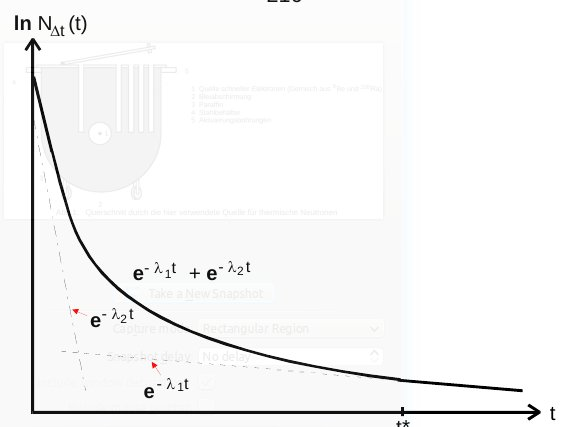
\includegraphics[scale=0.5]{pics/zerfall.jpeg}
	\caption{Beispiel für überlagerte Aktivität von zwei Isotopen - entnommen aus Versuchsanleitung}
\end{figure}

	\section{Durchführung}
	\subsection{Aparatur}
Für die Messungen wird ein Geigermüller-Zählrohr mit zwei separaten Zählern genutzt. Zusätzlich steckt es in einer Abschirmung aus Blei um die Nullrate zu minimieren.

\begin{figure}[htbp]
	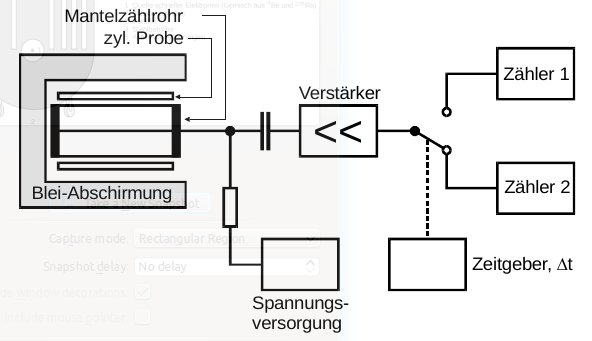
\includegraphics[scale=0.5]{pics/geiger.jpeg}
	\caption{Verwendetes Geiger-Müller-Zählrohr mit angeschlossenen Zählern - entnommen aus Versuchsanleitung}
\end{figure}
Das Geiger-Müller-Zählrohr besteht aus einer zylinderförmigen Kathode, in deren Mitte die stabförmige Anode steckt. Tritt Strahlung durch das Sichtfenster in das Zählrohr, so ionisiert diese Moleküle. Diese werden dann durch die angelegte Spannung zur Anode bzw. Kathode beschleunigt und ihr Auftreffen wird durch ein elektrisches Signal registriert.\\
Nach einer frei wählbaren Messzeit wechselt der Zählkanal, so dass der eben gemessene Wert abgelesen und trotzdem weitergezählt werden kann.

	\subsection{Versuch}
Bei der Durchführung wurde zunächst die sog. Nullrate bestimmt. Dies ist die Grundradioaktivität, die ständig um uns herum herrscht. Da sie die Ergebnisse verfälschen würde, wird sie im Voraus über einen sehr langen Zeitraum gemessen und danach bei jeder Messung von dem Ergebnis abgezogen.
Anschließend wurden eine Probe aus Indium und eine aus Rhodium aktiviert und über eine Dauer von 60 bzw 12 min ihre Aktivität gemessen.

	\section{Auswertung}

	\section{Diskussion}


% ========================================
%	Literaturverzeichnis
% ========================================

%\bibliographystyle{plainnat}			% Bibliographie-Style auswählen
%\bibliography{BIBDATEI}			% Literaturverzeichnis

% ========================================
%	Das Dokument endent
% ========================================

\end{document}
